\chapter{Young Entrepreneur Interviews Patrick Bet-David}

This interview from School of Hard Knocks, curated here by LazyingArt LLC, is not a blackboard lecture in the usual sense, but it does have a genuine mathematical spine. The speaker keeps translating experience into counts, thresholds, growth categories, purchase prices, valuation discounts, and simple decision rules. The safest way to write it is to follow the transcript in order: scale before explanation, focus before diversification, operator before valuation, liquidity before opportunity, audience fit before media scale, and finally belief before action.

\section{A Teaser of Scale}

The lecture opens by spending the conclusion first. Before we are told how the business was built, we are shown the later peaks: a year of extraordinary income, a mansion auction told through a funnel of hard numbers, and a terse thesis about cash. The cold open is therefore not yet an argument. It is a list of endpoints, meant to force the question of mechanism.

The arithmetic of the opening is simple and memorable:
\begin{align}
Y_{\max} &= \$250\,\text{million},\\
N_{\text{interest}} &= 4400,\qquad N_{\text{NDA}} = 131,\qquad D_{\text{bid}} = \$1\,\text{million},\\
P_{\text{buy}} &= \$25.2\,\text{million cash}.
\end{align}
What matters here is not only the magnitude of the numbers, but the order in which they are presented. We are shown scale and optionality before we are shown the thought that produced them.

Only after this teaser does the host reset the scene in Miami and promise a masterclass on business, sales, negotiation, and money. That reset is important. It tells us that the lecture will not remain at the level of spectacle. We are meant to ask how these numbers become possible.

\section{Concentration Before Diversification}

When the proper interview begins, the first doctrine arrives quickly. Bet-David says he first built wealth in insurance and only later moved into media and consulting. He then gives the lecture's first slogan: concentration builds wealth, diversification keeps it. The point is not merely motivational. It is operational. A company scales more easily when it does not diffuse its attention across many adjacent products.

His threshold for diversification is intentionally rough:
\begin{equation}
W_{\text{diversify}} \gtrsim \$10\,\text{billion}.
\end{equation}
The transcript does not tell us exactly what this threshold measures: personal wealth, company scale, or some broader level of economic security. We should therefore keep it speaker-attributed and approximate.

The supporting story is the Blue Ocean episode. He describes entering insurance, reading \emph{Blue Ocean Strategy}, gathering people in an emergency meeting, and then eliminating disability, stocks, bonds, mutual funds, variable annuities, and everything else that distracted from the core offer. The transcript contains a garbled phrase about licenses, but the clean payload is clear enough: he chose to use none of the surrounding options and to keep only life insurance.

The numerical evidence is the simplest equation in the section:
\begin{equation}
N_{\text{agents}} : 66 \longrightarrow 60{,}000.
\end{equation}
This is the lecture's first real proof by scale. Focus is not defended abstractly; it is defended by the growth of the machine after sprawl was cut away.

\subsection{Question \& Answer}

\paragraph{Question.} Why does narrowing the business create scale rather than limit it?

\paragraph{Answer.} In the lecture's logic, narrowing does not reduce possibility; it reduces friction. The organization learns one offer more deeply, trains around one value proposition, and compounds repetition rather than dissipating effort across loosely related products. We are not told that diversification is always wrong. We are told that it is early diversification that often destroys compounding.

\section{The Operator as the Limiting Variable}

The next move is from the business model to the person running it. The host asks about failure and longevity, and Bet-David answers with one of the lecture's strongest causal claims: everything rises and falls on the operator. The statistic that introduces the section is itself rough but memorable:
\begin{equation}
p_{\text{fail},5\text{yr}} \approx \frac{8}{10}.
\end{equation}
The speaker then relocates the explanation from the market to the operator.

A useful way to compress the lecture's claim is to bundle the speaker's variables together:
\begin{equation}
\mathcal{O}=\{\text{focus},\ \text{emotional stability},\ \text{feedback judgment}\}.
\end{equation}
The point is not that these variables are measured numerically in the interview. The point is that they are treated as the hidden state of the firm. If the operator is distracted, emotionally unstable, or unable to distinguish good feedback from prestigious but destructive feedback, then the company loses direction.

This is where the lecture's discussion of culture enters. Bet-David gives the example of a founder hiring someone with a Harvard degree and then surrendering too much authority to that credential. The danger is not education as such. The danger is allowing borrowed prestige to dissolve the culture that made the company function in the first place.

We can summarize the section in the speaker's own causal form:
\begin{equation}
\text{operator weakness} \Rightarrow \text{scaling difficulty}.
\end{equation}

\subsection{Question \& Answer}

\paragraph{Question.} How does a founder take feedback without letting outside prestige dissolve the company's culture?

\paragraph{Answer.} The lecture's answer is that feedback must be filtered through the company's purpose, not through the status of the person who offers it. Degrees do not automatically authorize cultural redesign. The operator must decide not simply whether advice is intelligent, but whether it is aligned with the machine he is trying to preserve and scale.

\section{Interruption and the CEO Problem}

Midway through the early business discussion, the interview is interrupted by the host's School of Mentors promotion. Structurally this matters, because the lecture does not move in a perfectly smooth argumentative line. It is a YouTube interview, and so its business doctrine is broken by the host's own business ecosystem. We should preserve that interruption as part of the rhythm, but keep it analytically separate.

When the interview resumes, the question is sharper than before: what took the business from eight to nine figures? Bet-David answers first by confessing a limit. At around
\begin{equation}
Y \approx \$10\,\text{million/year},
\end{equation}
he felt that he was strong in sales and disciplined with money, but not yet a real operator. This is a good moment in the lecture, because it admits that sales success and CEO competence are not identical.

The solution enters through Harvard OPM:
\begin{equation}
N_{\text{CEO}}=144,\qquad N_{\text{countries}}=64.
\end{equation}
There he meets a much larger operator, described as the Victoria's Secret analogue for New Zealand and Australia, whose scale is stated as
\begin{equation}
W_{\text{peer}} \approx \$1.5\,\text{billion},\qquad
N_{\text{employees}}=7000,\qquad
N_{\text{CEO reports}}=6.
\end{equation}
The peer then gives the lecture's central framework. No board survives, so we should reconstruct it cautiously from the spoken sequence rather than pretend we possess a diagram that was never validated. The scheme is:
\begin{equation}
G_{\text{linear}}=\{\text{biz dev},\ \text{systems}\},\qquad
G_{\text{exp}}=\{\text{leadership development},\ \text{innovative campaigns}\}.
\end{equation}
The hierarchy the speaker implies is
\begin{equation}
G_{\text{exp}} > G_{\text{linear}}
\qquad\text{for explosive upside.}
\end{equation}
This does not mean linear growth is useless. It means that business development, systems, and networking extend the current machine, while leadership development and genuinely original campaigns can change its scale regime.

\begin{figure}[h]
\centering
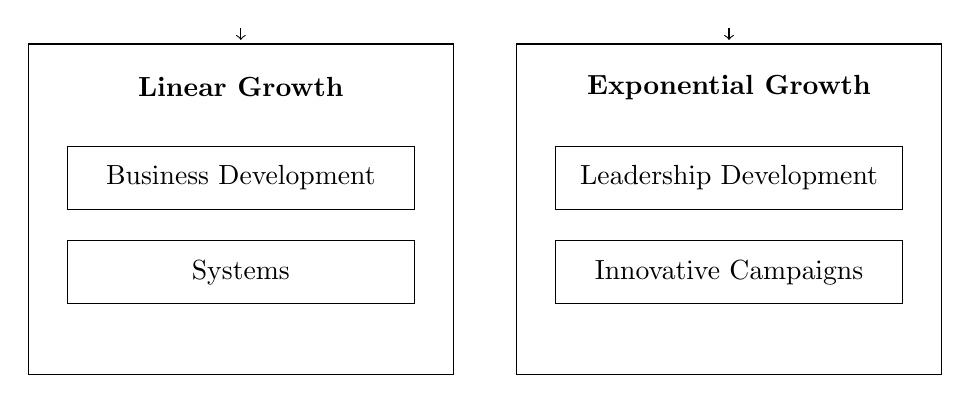
\begin{tikzpicture}
\draw (0,0) rectangle (5.4,4.2);
\draw (6.2,0) rectangle (11.6,4.2);

\node at (2.7,3.65) {\textbf{Linear Growth}};
\node at (8.9,3.65) {\textbf{Exponential Growth}};

\draw (0.5,2.9) rectangle (4.9,2.1);
\draw (0.5,1.7) rectangle (4.9,0.9);

\draw (6.7,2.9) rectangle (11.1,2.1);
\draw (6.7,1.7) rectangle (11.1,0.9);

\node at (2.7,2.5) {Business Development};
\node at (2.7,1.3) {Systems};

\node at (8.9,2.5) {Leadership Development};
\node at (8.9,1.3) {Innovative Campaigns};

\draw[->] (2.7,4.4) -- (2.7,4.25);
\draw[->] (8.9,4.4) -- (8.9,4.25);
\end{tikzpicture}
\caption{A cautious transcript-led reconstruction of the four growth levers described in the Harvard OPM story.}
\end{figure}

The Coke example, ``share a Coke with John,'' is valuable here because it shows what the speaker means by innovation. He does not mean innovation in the thin technological sense. He means a campaign that changes who buys, and why.

\subsection{Question \& Answer}

\paragraph{Question.} Why do systems and business development help a company grow without necessarily making it explode?

\paragraph{Answer.} Because they improve the efficiency and reach of the existing machine without altering its scale law. Systems make repetition cleaner; business development extends the present sales process. Leadership development and innovative campaigns, by contrast, can alter the structure of the organization or the market's perception of it, and so can produce discontinuous jumps.

\section{Cash as Optionality}

After growth comes treasury. Asked for the best financial advice he ever received, Bet-David answers: always have cash. This is not presented as a timid or defensive principle. It is presented as optionality.

The first example is the Wayne Gretzky card story:
\begin{align}
P_0 &= \$540{,}000,\\
V_{1.5\text{ yr}} &= \$2.2\,\text{million},\\
M &= \frac{V_{1.5\text{ yr}}}{P_0} \approx 4.07.
\end{align}
The lecture is not asking us to become sports-card traders. The mechanism is simpler. A distressed seller needs liquidity immediately. If we can transact now, we buy timing asymmetry.

The real-estate example is even cleaner because the auction process is visible in stages:
\begin{align}
P_{2018} &= \$25\,\text{million},\qquad
C_{\text{finish}} = \$7\,\text{million},\\
N_{\text{interest}} &= 4400,\qquad
N_{\text{NDA}} = 131,\qquad
D_{\text{bid}} = \$1\,\text{million},\\
P_{\text{buy}} &= \$25.2\,\text{million cash},\qquad
V_{\text{est}} \approx \$40\text{--}50\,\text{million}.
\end{align}
We can pull two worked comparisons out of the transcript. First, relative to the previous owner's basis,
\begin{align}
B_{\text{old owner}} &= P_{2018}+C_{\text{finish}} = 25+7 = \$32\,\text{million},\\
B_{\text{old owner}} - P_{\text{buy}} &= 32-25.2 = \$6.8\,\text{million}.
\end{align}
Second, relative to the speaker's own estimated value,
\begin{align}
\Delta V_{\text{low}} &= 40-25.2 = \$14.8\,\text{million},\\
\Delta V_{\text{high}} &= 50-25.2 = \$24.8\,\text{million}.
\end{align}
The estimate is not an audited appraisal, and so we should not overstate it. But the structure is clear enough. Cash is being modeled as the capacity to buy below someone else's need.

The doctrine may be compressed as
\begin{equation}
C_{\text{available}}+\text{market stress}\Rightarrow \text{mispricing access}.
\end{equation}
That is the heart of the section.

\section{The Market Tests the Message}

The lecture then turns from treasury to media. The host raises a sharp tension: great businessmen are often terrible content creators, and great content creators are often terrible businessmen. Bet-David's answer is not to romanticize either side. He says the market tells us whether we know what we are doing.

The key numerical story is an early failure:
\begin{equation}
t_{\text{early}} \approx 2\,\text{years},\qquad
N_{\text{subscribers}} \approx 1000.
\end{equation}
The point is brutal and useful. For roughly two years, almost nobody watched. The channel existed, but the market had not granted it fit.

The adjustment was not random creativity. It was narrowing. At an event he was told to pick one word, and the word became business and entrepreneurship. Titles then became disciplined variations on that niche: raising money as an entrepreneur, hiring as an entrepreneur, firing as an entrepreneur. The claimed later result is
\begin{equation}
s_{\text{page1}} \approx 50\%.
\end{equation}
That is, roughly half of the page-one results in the relevant search space were theirs.

The lecture's media rule is therefore
\begin{equation}
\text{market response}\Rightarrow \text{proof or refutation of message fit}.
\end{equation}
The market here is not mystical. It is search, click, watch time, repetition, and discoverability.

The speaker also suggests a simple communication taxonomy:
\begin{equation}
\mathcal{M}=\{\text{speaking},\ \text{video},\ \text{writing}\}.
\end{equation}
This should remain heuristic. The claim is that most people have some viable channel for getting their message into the world, but not every channel fits every person.

\subsection{Question \& Answer}

\paragraph{Question.} What does it mean for the market to tell us whether our message actually works?

\paragraph{Answer.} It means that self-evaluation is not enough. We may think we communicate clearly, but the test is whether people search, stop, watch, and return. In the lecture, two years of weak response are treated not as bad luck but as a failed experiment. Narrower language and repeated title discipline then become the next experiment, and the market's later response is taken as a partial proof.

\section{Needs Analysis, Desperation, and Valuation}

From media the lecture moves back into selling, and here Bet-David's doctrine is simple: needs analysis. We must discover what matters to the other side before we decide what to recommend. His examples come first from his children and then from clients, but the formal structure is the same:
\begin{equation}
R^*=\arg\max_R \operatorname{Fit}(R,\text{buyer priorities}).
\end{equation}
A recommendation chosen before the buyer's priorities are known is merely a projection of the seller's habits. This is why the lecture repeatedly returns to questions rather than scripts.

The same logic of structure over impulse carries into negotiation. The rule there is
\begin{equation}
\text{desperation}\Rightarrow \text{underpricing}+\text{bad decisions}.
\end{equation}
The company-sale story is the lecture's sharpest proof. A first buyer offers
\begin{equation}
V_1=\$120\,\text{million},\qquad
U_1=50\%\ \text{upfront},\qquad
T_{\text{stay}}=5\,\text{years}.
\end{equation}
The reason is revealing: employees all say Bet-David is the hardest-working person in the company, and so the buyer concludes that the firm is really founder labor disguised as a company. In the lecture's own language, they cannot buy the business because he is running the company.

This gives us a useful discount rule:
\begin{equation}
\text{founder-centric operation}\Rightarrow \text{valuation discount}.
\end{equation}
The response is not rhetorical bargaining. It is redesign. He moves to Florida, hires
\begin{equation}
N_{\text{new C-suite}} = 5
\end{equation}
new executives, lets them run the business, and waits
\begin{equation}
t_{\text{wait}} = 2\,\text{years}.
\end{equation}
Then, when the next due-diligence round comes, employees say he is only there occasionally. The firm now looks like a transferable machine. The transcript's payoff is that the later valuation exceeded twice the first one:
\begin{align}
V_2 &> 2V_1,\\
V_2 &> 2 \times \$120\,\text{million} = \$240\,\text{million}.
\end{align}
This lower bound is worth writing explicitly. It shows how large the price effect of founder decoupling can be in the lecture's own arithmetic.

\subsection{Question \& Answer}

\paragraph{Question.} Why can removing the founder from daily operations increase valuation more than simply working harder inside the company?

\paragraph{Answer.} Because an acquirer buys transferable structure, not merely admirable effort. If the company's earnings depend on one person's constant presence, then the buyer is purchasing fragility. Once management is distributed and repeatable, the company becomes legible as an asset rather than as personal exertion. In that form it commands a different price.

\section{Summary}

The lecture closes by moving from commercial structure to philosophy. Asked what separates middle-class thinking from long-term wealth building, Bet-David answers by refusing inherited beliefs that do not survive questioning. The final message broadens the same rule: information is now widely accessible, and so many excuses that once looked like destiny should now be treated as beliefs to be examined rather than facts to be obeyed.

We can summarize the chapter in a short chain of implications:
\begin{align}
\text{concentration} &\Rightarrow \text{compounding focus},\\
\text{operator quality} &\Rightarrow \text{organizational durability},\\
\text{cash} &\Rightarrow \text{optionality under stress},\\
\text{message-market fit} &\Rightarrow \text{media scale},\\
\text{founder decoupling} &\Rightarrow \text{higher valuation},\\
\text{belief revision} &\Rightarrow \text{commercial revision}.
\end{align}
That is the real order of the lecture. It begins with spectacular numbers, but it ends by arguing that numbers are downstream of structure: the right focus, the right operator, the right balance sheet, the right message, the right company architecture, and finally the right refusal of inherited limits.